\documentclass[tikz,border=4pt]{standalone}
\usepackage{amsmath}
\usepackage{tikz}
\usetikzlibrary{arrows.meta,positioning,fit,backgrounds,calc,shapes.geometric,decorations.pathreplacing,patterns}
\usepackage{xcolor}
\renewcommand{\familydefault}{\sfdefault}
\definecolor{cdata}{HTML}{1F5FA8}
\definecolor{cctrl}{HTML}{15796F}
\definecolor{cres}{HTML}{6A4C93}
\definecolor{cgray}{HTML}{5A6570}
\definecolor{cwarn}{HTML}{B4561B}
\tikzset{
  base/.style={rounded corners=1.8pt, line width=0.6pt, align=center, font=\scriptsize, inner sep=3pt, minimum height=8mm, text=black!85},
  data/.style={base, draw=cdata, fill=cdata!9},
  ctrl/.style={base, draw=cctrl, fill=cctrl!9},
  res/.style={base, draw=cres, fill=cres!9},
  art/.style={base, draw=black!65, fill=black!7},
  ext/.style={base, draw=cgray, fill=white, dashed},
  gate/.style={font=\tiny\bfseries, text=cwarn, draw=cwarn, rounded corners=1pt, inner sep=1.6pt, fill=white, line width=0.5pt},
  arr/.style={-{Stealth[length=2.0mm,width=1.5mm]}, line width=0.6pt, draw=cgray!85!black},
  arr2/.style={{Stealth[length=2.0mm,width=1.5mm]}-{Stealth[length=2.0mm,width=1.5mm]}, line width=0.6pt, draw=cgray!85!black},
  darr/.style={-{Stealth[length=2.0mm,width=1.5mm]}, line width=0.6pt, dashed, draw=cgray!85!black},
  lbl/.style={font=\tiny, text=cgray!90!black, inner sep=1pt},
  band/.style={rounded corners=3pt, line width=0.7pt},
}
\newcommand{\dotsep}{\,$\cdot$\,}
\renewcommand{\tiny}{\fontsize{6}{7}\selectfont}

\definecolor{p0}{HTML}{0072B2}
\definecolor{p1}{HTML}{E69F00}
\definecolor{p2}{HTML}{009E73}
\definecolor{p3}{HTML}{D55E00}
\definecolor{p4}{HTML}{CC79A7}
\begin{document}
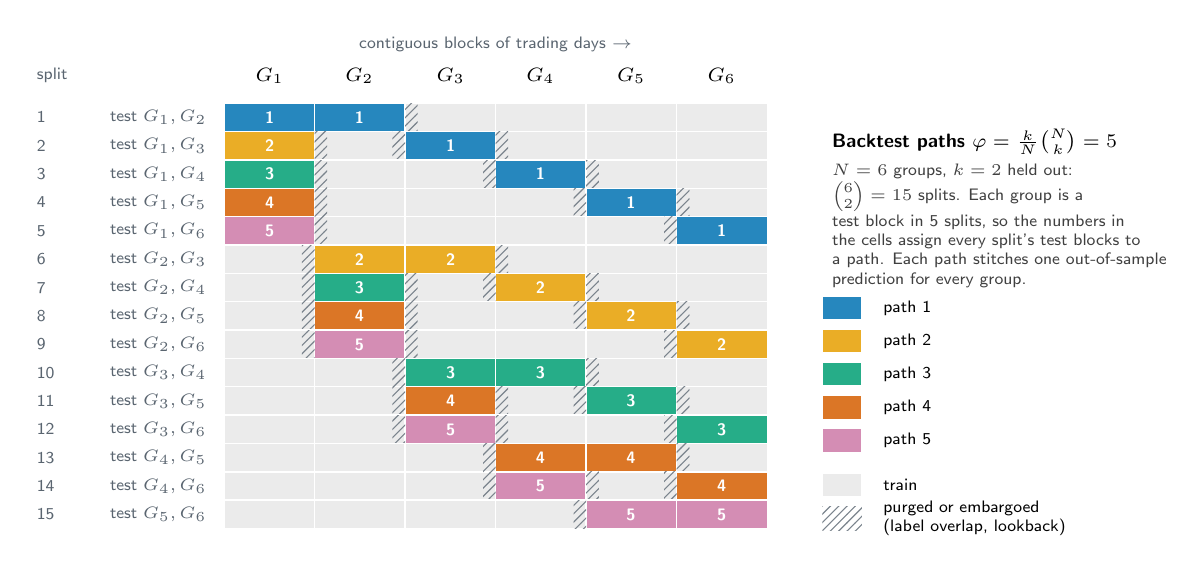
\begin{tikzpicture}
\node[font=\scriptsize\bfseries] at (2.58,0.35) {$G_1$};
\node[font=\scriptsize\bfseries] at (3.72,0.35) {$G_2$};
\node[font=\scriptsize\bfseries] at (4.88,0.35) {$G_3$};
\node[font=\scriptsize\bfseries] at (6.02,0.35) {$G_4$};
\node[font=\scriptsize\bfseries] at (7.17,0.35) {$G_5$};
\node[font=\scriptsize\bfseries] at (8.32,0.35) {$G_6$};
\node[font=\tiny, text=cgray] at (5.45,0.75) {contiguous blocks of trading days $\rightarrow$};
\node[font=\tiny, anchor=west, text=cgray] at (-0.5,0.35) {split};
\node[font=\tiny, anchor=west, text=cgray] at (-0.5,-0.18) {1};
\node[font=\tiny, anchor=east, text=cgray] at (1.90,-0.18) {test $G_1,G_2$};
\draw[fill=p0!85, draw=white, line width=0.5pt] (2.00,-0.36) rectangle (3.15,0.00);
\node[font=\tiny\bfseries, text=white] at (2.58,-0.18) {1};
\draw[fill=p0!85, draw=white, line width=0.5pt] (3.15,-0.36) rectangle (4.30,0.00);
\node[font=\tiny\bfseries, text=white] at (3.72,-0.18) {1};
\draw[fill=black!8, draw=white, line width=0.5pt] (4.30,-0.36) rectangle (5.45,0.00);
\draw[fill=black!8, draw=white, line width=0.5pt] (5.45,-0.36) rectangle (6.60,0.00);
\draw[fill=black!8, draw=white, line width=0.5pt] (6.60,-0.36) rectangle (7.75,0.00);
\draw[fill=black!8, draw=white, line width=0.5pt] (7.75,-0.36) rectangle (8.90,0.00);
\fill[pattern=north east lines, pattern color=cgray!80] (4.30,-0.36) rectangle (4.46,0.00);
\node[font=\tiny, anchor=west, text=cgray] at (-0.5,-0.54) {2};
\node[font=\tiny, anchor=east, text=cgray] at (1.90,-0.54) {test $G_1,G_3$};
\draw[fill=p1!85, draw=white, line width=0.5pt] (2.00,-0.72) rectangle (3.15,-0.36);
\node[font=\tiny\bfseries, text=white] at (2.58,-0.54) {2};
\draw[fill=black!8, draw=white, line width=0.5pt] (3.15,-0.72) rectangle (4.30,-0.36);
\draw[fill=p0!85, draw=white, line width=0.5pt] (4.30,-0.72) rectangle (5.45,-0.36);
\node[font=\tiny\bfseries, text=white] at (4.88,-0.54) {1};
\draw[fill=black!8, draw=white, line width=0.5pt] (5.45,-0.72) rectangle (6.60,-0.36);
\draw[fill=black!8, draw=white, line width=0.5pt] (6.60,-0.72) rectangle (7.75,-0.36);
\draw[fill=black!8, draw=white, line width=0.5pt] (7.75,-0.72) rectangle (8.90,-0.36);
\fill[pattern=north east lines, pattern color=cgray!80] (3.15,-0.72) rectangle (3.31,-0.36);
\fill[pattern=north east lines, pattern color=cgray!80] (4.14,-0.72) rectangle (4.30,-0.36);
\fill[pattern=north east lines, pattern color=cgray!80] (5.45,-0.72) rectangle (5.61,-0.36);
\node[font=\tiny, anchor=west, text=cgray] at (-0.5,-0.90) {3};
\node[font=\tiny, anchor=east, text=cgray] at (1.90,-0.90) {test $G_1,G_4$};
\draw[fill=p2!85, draw=white, line width=0.5pt] (2.00,-1.08) rectangle (3.15,-0.72);
\node[font=\tiny\bfseries, text=white] at (2.58,-0.90) {3};
\draw[fill=black!8, draw=white, line width=0.5pt] (3.15,-1.08) rectangle (4.30,-0.72);
\draw[fill=black!8, draw=white, line width=0.5pt] (4.30,-1.08) rectangle (5.45,-0.72);
\draw[fill=p0!85, draw=white, line width=0.5pt] (5.45,-1.08) rectangle (6.60,-0.72);
\node[font=\tiny\bfseries, text=white] at (6.02,-0.90) {1};
\draw[fill=black!8, draw=white, line width=0.5pt] (6.60,-1.08) rectangle (7.75,-0.72);
\draw[fill=black!8, draw=white, line width=0.5pt] (7.75,-1.08) rectangle (8.90,-0.72);
\fill[pattern=north east lines, pattern color=cgray!80] (3.15,-1.08) rectangle (3.31,-0.72);
\fill[pattern=north east lines, pattern color=cgray!80] (5.29,-1.08) rectangle (5.45,-0.72);
\fill[pattern=north east lines, pattern color=cgray!80] (6.60,-1.08) rectangle (6.76,-0.72);
\node[font=\tiny, anchor=west, text=cgray] at (-0.5,-1.26) {4};
\node[font=\tiny, anchor=east, text=cgray] at (1.90,-1.26) {test $G_1,G_5$};
\draw[fill=p3!85, draw=white, line width=0.5pt] (2.00,-1.44) rectangle (3.15,-1.08);
\node[font=\tiny\bfseries, text=white] at (2.58,-1.26) {4};
\draw[fill=black!8, draw=white, line width=0.5pt] (3.15,-1.44) rectangle (4.30,-1.08);
\draw[fill=black!8, draw=white, line width=0.5pt] (4.30,-1.44) rectangle (5.45,-1.08);
\draw[fill=black!8, draw=white, line width=0.5pt] (5.45,-1.44) rectangle (6.60,-1.08);
\draw[fill=p0!85, draw=white, line width=0.5pt] (6.60,-1.44) rectangle (7.75,-1.08);
\node[font=\tiny\bfseries, text=white] at (7.17,-1.26) {1};
\draw[fill=black!8, draw=white, line width=0.5pt] (7.75,-1.44) rectangle (8.90,-1.08);
\fill[pattern=north east lines, pattern color=cgray!80] (3.15,-1.44) rectangle (3.31,-1.08);
\fill[pattern=north east lines, pattern color=cgray!80] (6.44,-1.44) rectangle (6.60,-1.08);
\fill[pattern=north east lines, pattern color=cgray!80] (7.75,-1.44) rectangle (7.91,-1.08);
\node[font=\tiny, anchor=west, text=cgray] at (-0.5,-1.62) {5};
\node[font=\tiny, anchor=east, text=cgray] at (1.90,-1.62) {test $G_1,G_6$};
\draw[fill=p4!85, draw=white, line width=0.5pt] (2.00,-1.80) rectangle (3.15,-1.44);
\node[font=\tiny\bfseries, text=white] at (2.58,-1.62) {5};
\draw[fill=black!8, draw=white, line width=0.5pt] (3.15,-1.80) rectangle (4.30,-1.44);
\draw[fill=black!8, draw=white, line width=0.5pt] (4.30,-1.80) rectangle (5.45,-1.44);
\draw[fill=black!8, draw=white, line width=0.5pt] (5.45,-1.80) rectangle (6.60,-1.44);
\draw[fill=black!8, draw=white, line width=0.5pt] (6.60,-1.80) rectangle (7.75,-1.44);
\draw[fill=p0!85, draw=white, line width=0.5pt] (7.75,-1.80) rectangle (8.90,-1.44);
\node[font=\tiny\bfseries, text=white] at (8.32,-1.62) {1};
\fill[pattern=north east lines, pattern color=cgray!80] (3.15,-1.80) rectangle (3.31,-1.44);
\fill[pattern=north east lines, pattern color=cgray!80] (7.59,-1.80) rectangle (7.75,-1.44);
\node[font=\tiny, anchor=west, text=cgray] at (-0.5,-1.98) {6};
\node[font=\tiny, anchor=east, text=cgray] at (1.90,-1.98) {test $G_2,G_3$};
\draw[fill=black!8, draw=white, line width=0.5pt] (2.00,-2.16) rectangle (3.15,-1.80);
\draw[fill=p1!85, draw=white, line width=0.5pt] (3.15,-2.16) rectangle (4.30,-1.80);
\node[font=\tiny\bfseries, text=white] at (3.72,-1.98) {2};
\draw[fill=p1!85, draw=white, line width=0.5pt] (4.30,-2.16) rectangle (5.45,-1.80);
\node[font=\tiny\bfseries, text=white] at (4.88,-1.98) {2};
\draw[fill=black!8, draw=white, line width=0.5pt] (5.45,-2.16) rectangle (6.60,-1.80);
\draw[fill=black!8, draw=white, line width=0.5pt] (6.60,-2.16) rectangle (7.75,-1.80);
\draw[fill=black!8, draw=white, line width=0.5pt] (7.75,-2.16) rectangle (8.90,-1.80);
\fill[pattern=north east lines, pattern color=cgray!80] (2.99,-2.16) rectangle (3.15,-1.80);
\fill[pattern=north east lines, pattern color=cgray!80] (5.45,-2.16) rectangle (5.61,-1.80);
\node[font=\tiny, anchor=west, text=cgray] at (-0.5,-2.34) {7};
\node[font=\tiny, anchor=east, text=cgray] at (1.90,-2.34) {test $G_2,G_4$};
\draw[fill=black!8, draw=white, line width=0.5pt] (2.00,-2.52) rectangle (3.15,-2.16);
\draw[fill=p2!85, draw=white, line width=0.5pt] (3.15,-2.52) rectangle (4.30,-2.16);
\node[font=\tiny\bfseries, text=white] at (3.72,-2.34) {3};
\draw[fill=black!8, draw=white, line width=0.5pt] (4.30,-2.52) rectangle (5.45,-2.16);
\draw[fill=p1!85, draw=white, line width=0.5pt] (5.45,-2.52) rectangle (6.60,-2.16);
\node[font=\tiny\bfseries, text=white] at (6.02,-2.34) {2};
\draw[fill=black!8, draw=white, line width=0.5pt] (6.60,-2.52) rectangle (7.75,-2.16);
\draw[fill=black!8, draw=white, line width=0.5pt] (7.75,-2.52) rectangle (8.90,-2.16);
\fill[pattern=north east lines, pattern color=cgray!80] (2.99,-2.52) rectangle (3.15,-2.16);
\fill[pattern=north east lines, pattern color=cgray!80] (4.30,-2.52) rectangle (4.46,-2.16);
\fill[pattern=north east lines, pattern color=cgray!80] (5.29,-2.52) rectangle (5.45,-2.16);
\fill[pattern=north east lines, pattern color=cgray!80] (6.60,-2.52) rectangle (6.76,-2.16);
\node[font=\tiny, anchor=west, text=cgray] at (-0.5,-2.70) {8};
\node[font=\tiny, anchor=east, text=cgray] at (1.90,-2.70) {test $G_2,G_5$};
\draw[fill=black!8, draw=white, line width=0.5pt] (2.00,-2.88) rectangle (3.15,-2.52);
\draw[fill=p3!85, draw=white, line width=0.5pt] (3.15,-2.88) rectangle (4.30,-2.52);
\node[font=\tiny\bfseries, text=white] at (3.72,-2.70) {4};
\draw[fill=black!8, draw=white, line width=0.5pt] (4.30,-2.88) rectangle (5.45,-2.52);
\draw[fill=black!8, draw=white, line width=0.5pt] (5.45,-2.88) rectangle (6.60,-2.52);
\draw[fill=p1!85, draw=white, line width=0.5pt] (6.60,-2.88) rectangle (7.75,-2.52);
\node[font=\tiny\bfseries, text=white] at (7.17,-2.70) {2};
\draw[fill=black!8, draw=white, line width=0.5pt] (7.75,-2.88) rectangle (8.90,-2.52);
\fill[pattern=north east lines, pattern color=cgray!80] (2.99,-2.88) rectangle (3.15,-2.52);
\fill[pattern=north east lines, pattern color=cgray!80] (4.30,-2.88) rectangle (4.46,-2.52);
\fill[pattern=north east lines, pattern color=cgray!80] (6.44,-2.88) rectangle (6.60,-2.52);
\fill[pattern=north east lines, pattern color=cgray!80] (7.75,-2.88) rectangle (7.91,-2.52);
\node[font=\tiny, anchor=west, text=cgray] at (-0.5,-3.06) {9};
\node[font=\tiny, anchor=east, text=cgray] at (1.90,-3.06) {test $G_2,G_6$};
\draw[fill=black!8, draw=white, line width=0.5pt] (2.00,-3.24) rectangle (3.15,-2.88);
\draw[fill=p4!85, draw=white, line width=0.5pt] (3.15,-3.24) rectangle (4.30,-2.88);
\node[font=\tiny\bfseries, text=white] at (3.72,-3.06) {5};
\draw[fill=black!8, draw=white, line width=0.5pt] (4.30,-3.24) rectangle (5.45,-2.88);
\draw[fill=black!8, draw=white, line width=0.5pt] (5.45,-3.24) rectangle (6.60,-2.88);
\draw[fill=black!8, draw=white, line width=0.5pt] (6.60,-3.24) rectangle (7.75,-2.88);
\draw[fill=p1!85, draw=white, line width=0.5pt] (7.75,-3.24) rectangle (8.90,-2.88);
\node[font=\tiny\bfseries, text=white] at (8.32,-3.06) {2};
\fill[pattern=north east lines, pattern color=cgray!80] (2.99,-3.24) rectangle (3.15,-2.88);
\fill[pattern=north east lines, pattern color=cgray!80] (4.30,-3.24) rectangle (4.46,-2.88);
\fill[pattern=north east lines, pattern color=cgray!80] (7.59,-3.24) rectangle (7.75,-2.88);
\node[font=\tiny, anchor=west, text=cgray] at (-0.5,-3.42) {10};
\node[font=\tiny, anchor=east, text=cgray] at (1.90,-3.42) {test $G_3,G_4$};
\draw[fill=black!8, draw=white, line width=0.5pt] (2.00,-3.60) rectangle (3.15,-3.24);
\draw[fill=black!8, draw=white, line width=0.5pt] (3.15,-3.60) rectangle (4.30,-3.24);
\draw[fill=p2!85, draw=white, line width=0.5pt] (4.30,-3.60) rectangle (5.45,-3.24);
\node[font=\tiny\bfseries, text=white] at (4.88,-3.42) {3};
\draw[fill=p2!85, draw=white, line width=0.5pt] (5.45,-3.60) rectangle (6.60,-3.24);
\node[font=\tiny\bfseries, text=white] at (6.02,-3.42) {3};
\draw[fill=black!8, draw=white, line width=0.5pt] (6.60,-3.60) rectangle (7.75,-3.24);
\draw[fill=black!8, draw=white, line width=0.5pt] (7.75,-3.60) rectangle (8.90,-3.24);
\fill[pattern=north east lines, pattern color=cgray!80] (4.14,-3.60) rectangle (4.30,-3.24);
\fill[pattern=north east lines, pattern color=cgray!80] (6.60,-3.60) rectangle (6.76,-3.24);
\node[font=\tiny, anchor=west, text=cgray] at (-0.5,-3.78) {11};
\node[font=\tiny, anchor=east, text=cgray] at (1.90,-3.78) {test $G_3,G_5$};
\draw[fill=black!8, draw=white, line width=0.5pt] (2.00,-3.96) rectangle (3.15,-3.60);
\draw[fill=black!8, draw=white, line width=0.5pt] (3.15,-3.96) rectangle (4.30,-3.60);
\draw[fill=p3!85, draw=white, line width=0.5pt] (4.30,-3.96) rectangle (5.45,-3.60);
\node[font=\tiny\bfseries, text=white] at (4.88,-3.78) {4};
\draw[fill=black!8, draw=white, line width=0.5pt] (5.45,-3.96) rectangle (6.60,-3.60);
\draw[fill=p2!85, draw=white, line width=0.5pt] (6.60,-3.96) rectangle (7.75,-3.60);
\node[font=\tiny\bfseries, text=white] at (7.17,-3.78) {3};
\draw[fill=black!8, draw=white, line width=0.5pt] (7.75,-3.96) rectangle (8.90,-3.60);
\fill[pattern=north east lines, pattern color=cgray!80] (4.14,-3.96) rectangle (4.30,-3.60);
\fill[pattern=north east lines, pattern color=cgray!80] (5.45,-3.96) rectangle (5.61,-3.60);
\fill[pattern=north east lines, pattern color=cgray!80] (6.44,-3.96) rectangle (6.60,-3.60);
\fill[pattern=north east lines, pattern color=cgray!80] (7.75,-3.96) rectangle (7.91,-3.60);
\node[font=\tiny, anchor=west, text=cgray] at (-0.5,-4.14) {12};
\node[font=\tiny, anchor=east, text=cgray] at (1.90,-4.14) {test $G_3,G_6$};
\draw[fill=black!8, draw=white, line width=0.5pt] (2.00,-4.32) rectangle (3.15,-3.96);
\draw[fill=black!8, draw=white, line width=0.5pt] (3.15,-4.32) rectangle (4.30,-3.96);
\draw[fill=p4!85, draw=white, line width=0.5pt] (4.30,-4.32) rectangle (5.45,-3.96);
\node[font=\tiny\bfseries, text=white] at (4.88,-4.14) {5};
\draw[fill=black!8, draw=white, line width=0.5pt] (5.45,-4.32) rectangle (6.60,-3.96);
\draw[fill=black!8, draw=white, line width=0.5pt] (6.60,-4.32) rectangle (7.75,-3.96);
\draw[fill=p2!85, draw=white, line width=0.5pt] (7.75,-4.32) rectangle (8.90,-3.96);
\node[font=\tiny\bfseries, text=white] at (8.32,-4.14) {3};
\fill[pattern=north east lines, pattern color=cgray!80] (4.14,-4.32) rectangle (4.30,-3.96);
\fill[pattern=north east lines, pattern color=cgray!80] (5.45,-4.32) rectangle (5.61,-3.96);
\fill[pattern=north east lines, pattern color=cgray!80] (7.59,-4.32) rectangle (7.75,-3.96);
\node[font=\tiny, anchor=west, text=cgray] at (-0.5,-4.50) {13};
\node[font=\tiny, anchor=east, text=cgray] at (1.90,-4.50) {test $G_4,G_5$};
\draw[fill=black!8, draw=white, line width=0.5pt] (2.00,-4.68) rectangle (3.15,-4.32);
\draw[fill=black!8, draw=white, line width=0.5pt] (3.15,-4.68) rectangle (4.30,-4.32);
\draw[fill=black!8, draw=white, line width=0.5pt] (4.30,-4.68) rectangle (5.45,-4.32);
\draw[fill=p3!85, draw=white, line width=0.5pt] (5.45,-4.68) rectangle (6.60,-4.32);
\node[font=\tiny\bfseries, text=white] at (6.02,-4.50) {4};
\draw[fill=p3!85, draw=white, line width=0.5pt] (6.60,-4.68) rectangle (7.75,-4.32);
\node[font=\tiny\bfseries, text=white] at (7.17,-4.50) {4};
\draw[fill=black!8, draw=white, line width=0.5pt] (7.75,-4.68) rectangle (8.90,-4.32);
\fill[pattern=north east lines, pattern color=cgray!80] (5.29,-4.68) rectangle (5.45,-4.32);
\fill[pattern=north east lines, pattern color=cgray!80] (7.75,-4.68) rectangle (7.91,-4.32);
\node[font=\tiny, anchor=west, text=cgray] at (-0.5,-4.86) {14};
\node[font=\tiny, anchor=east, text=cgray] at (1.90,-4.86) {test $G_4,G_6$};
\draw[fill=black!8, draw=white, line width=0.5pt] (2.00,-5.04) rectangle (3.15,-4.68);
\draw[fill=black!8, draw=white, line width=0.5pt] (3.15,-5.04) rectangle (4.30,-4.68);
\draw[fill=black!8, draw=white, line width=0.5pt] (4.30,-5.04) rectangle (5.45,-4.68);
\draw[fill=p4!85, draw=white, line width=0.5pt] (5.45,-5.04) rectangle (6.60,-4.68);
\node[font=\tiny\bfseries, text=white] at (6.02,-4.86) {5};
\draw[fill=black!8, draw=white, line width=0.5pt] (6.60,-5.04) rectangle (7.75,-4.68);
\draw[fill=p3!85, draw=white, line width=0.5pt] (7.75,-5.04) rectangle (8.90,-4.68);
\node[font=\tiny\bfseries, text=white] at (8.32,-4.86) {4};
\fill[pattern=north east lines, pattern color=cgray!80] (5.29,-5.04) rectangle (5.45,-4.68);
\fill[pattern=north east lines, pattern color=cgray!80] (6.60,-5.04) rectangle (6.76,-4.68);
\fill[pattern=north east lines, pattern color=cgray!80] (7.59,-5.04) rectangle (7.75,-4.68);
\node[font=\tiny, anchor=west, text=cgray] at (-0.5,-5.22) {15};
\node[font=\tiny, anchor=east, text=cgray] at (1.90,-5.22) {test $G_5,G_6$};
\draw[fill=black!8, draw=white, line width=0.5pt] (2.00,-5.40) rectangle (3.15,-5.04);
\draw[fill=black!8, draw=white, line width=0.5pt] (3.15,-5.40) rectangle (4.30,-5.04);
\draw[fill=black!8, draw=white, line width=0.5pt] (4.30,-5.40) rectangle (5.45,-5.04);
\draw[fill=black!8, draw=white, line width=0.5pt] (5.45,-5.40) rectangle (6.60,-5.04);
\draw[fill=p4!85, draw=white, line width=0.5pt] (6.60,-5.40) rectangle (7.75,-5.04);
\node[font=\tiny\bfseries, text=white] at (7.17,-5.22) {5};
\draw[fill=p4!85, draw=white, line width=0.5pt] (7.75,-5.40) rectangle (8.90,-5.04);
\node[font=\tiny\bfseries, text=white] at (8.32,-5.22) {5};
\fill[pattern=north east lines, pattern color=cgray!80] (6.44,-5.40) rectangle (6.60,-5.04);
\node[font=\scriptsize\bfseries, anchor=north west] at (9.60,-0.20) {Backtest paths $\varphi = \tfrac{k}{N}\binom{N}{k} = 5$};
\node[font=\tiny, anchor=north west, align=left, text=black!75] at (9.60,-0.65) {$N=6$ groups, $k=2$ held out:\\$\binom{6}{2}=15$ splits. Each group is a\\test block in 5 splits, so the numbers in\\the cells assign every split's test blocks to\\a path. Each path stitches one out-of-sample\\prediction for every group.};
\draw[fill=p0!85, draw=white] (9.60,-2.75) rectangle (10.10,-2.45);
\node[font=\tiny, anchor=west] at (10.25,-2.60) {path 1};
\draw[fill=p1!85, draw=white] (9.60,-3.17) rectangle (10.10,-2.87);
\node[font=\tiny, anchor=west] at (10.25,-3.02) {path 2};
\draw[fill=p2!85, draw=white] (9.60,-3.59) rectangle (10.10,-3.29);
\node[font=\tiny, anchor=west] at (10.25,-3.44) {path 3};
\draw[fill=p3!85, draw=white] (9.60,-4.01) rectangle (10.10,-3.71);
\node[font=\tiny, anchor=west] at (10.25,-3.86) {path 4};
\draw[fill=p4!85, draw=white] (9.60,-4.43) rectangle (10.10,-4.13);
\node[font=\tiny, anchor=west] at (10.25,-4.28) {path 5};
\draw[fill=black!8, draw=white] (9.60,-5.00) rectangle (10.10,-4.70);
\node[font=\tiny, anchor=west] at (10.25,-4.85) {train};
\fill[pattern=north east lines, pattern color=cgray!80] (9.60,-5.42) rectangle (10.10,-5.12);
\node[font=\tiny, anchor=west, align=left] at (10.25,-5.27) {purged or embargoed\\(label overlap, lookback)};
\end{tikzpicture}
\end{document}